

\documentclass{UNESC}
\usepackage[T1]{fontenc}
\usepackage[utf8]{inputenc}%\usepackage[latin1]{inputenc}
\renewcommand{\rmdefault}{phv} % Arial
\renewcommand{\sfdefault}{phv} % Arial
\usepackage[brazilian]{babel}
\usepackage{graphicx}
\usepackage{hyperref}
\usepackage{quoting}
\usepackage[labelsep=none]{caption}
\DeclareCaptionLabelFormat{figuracomtraco}{#1~#2 -}
\captionsetup[figure]{labelformat=figuracomtraco, labelsep=space}
\captionsetup[table]{labelformat=simple, labelsep=space, textformat=simple}
\DeclareCaptionLabelFormat{tabelacomtraco}{#1~#2 -}
\captionsetup[table]{labelformat=tabelacomtraco}
\captionsetup{labelsep=none}
\usepackage{enumitem}
\usepackage{float}
\usepackage{comment}
\usepackage[hang,flushmargin]{footmisc}
\usepackage{array}
\usepackage{adjustbox}
\setlength{\emergencystretch}{3em}

\hypersetup{
  setpagesize  = false,
  colorlinks   = true,    % Colours links instead of ugly boxes
  urlcolor     = blue,    % Colour for external hyperlinks
  linkcolor    = black,   % Colour of internal links
  citecolor    = black    % Colour of citations
}

\urlstyle{same}
\usepackage{setspace}

\usepackage[alf,recuo=0.0cm,abnt-emphasize=bf]{abntex2cite} 

\title{REGISTRO DIGITAL ANIMAL: DIGITALIZANDO A IDENTIFICAÇÃO E CONTROLE DE VACINAÇÃO DE ANIMAIS DE ESTIMAÇÃO}
\author
{
   Gabriel Goulart de Souza\footnote{Curso de Ciência da Computação, Universidade do Extremo Sul Catarinense (Unesc), Criciúma - Santa Catarina - Brasil. gabriel.gsouzza6@unesc.net},
   Diorgines Mattos Machado\footnote{Coorientador(a), Curso de Ciência da Computação, Universidade do Extremo Sul Catarinense (Unesc), Criciúma - Santa Catarina - Brasil. diorginesmattos@unesc.net},
   Allan Farias Favaro\footnote{Orientador(a), Curso de Ciência da Computação, Universidade do Extremo Sul Catarinense (Unesc), Criciúma - Santa Catarina - Brasil. allanfavaro@gmail.com}
}

\begin{document}

\onehalfspacing

\maketitle

\noindent
\textbf{Resumo:} A dispersão de informações de identificação, vacinação e documentos clínicos dificulta a organização e a consulta ao histórico dos animais de estimação. Este trabalho teve como objetivo desenvolver e avaliar o funcionamento de uma aplicação multiplataforma para cadastro, organização e consulta desses registros. Foi desenvolvida a aplicação Registro Digital Animal, com interface web progressiva, serviços de autenticação e sincronização e persistência no PostgreSQL. A avaliação reuniu 15 cenários funcionais de caixa-preta e a análise qualitativa de dois retornos preservados do setor veterinário, após 96 convites registrados e 13 aceites. Os cenários funcionais foram registrados como aprovados nas condições avaliadas, incluindo consulta a dados previamente armazenados e sincronização posterior. Os retornos apontaram utilidade na organização das informações e no planejamento de viagens, mas também identificaram dificuldade no preenchimento de peso decimal e oportunidades de aprimoramento dos campos de vacinação e da localização de clínicas. A pesquisa apresenta um artefato computacional e evidências exploratórias sobre sua adequação ao contexto de uso. A avaliação não mensurou redução do emprego de documentos físicos nem permite generalizar a usabilidade, devido ao alcance dos testes e ao conjunto reduzido de retornos disponíveis.

\vspace{0.5em}
\noindent
\textbf{Palavras-chave:} animais de estimação; registro digital; vacinação animal; aplicação web progressiva; testes funcionais.

\vspace{1.0em}
\noindent
\textbf{ABSTRACT:} Scattered identification, vaccination, and clinical documents make it difficult to organize and consult the records of companion animals. This study aimed to develop and evaluate the operation of a cross-platform application for registering, organizing, and consulting these records. The Registro Digital Animal application was developed with a progressive web interface, authentication and synchronization services, and PostgreSQL persistence. The evaluation combined 15 black-box functional scenarios with a qualitative analysis of two preserved responses from the veterinary sector, following 96 recorded invitations and 13 acceptances. The functional scenarios were recorded as passed under the evaluated conditions, including access to previously stored data and subsequent synchronization. The responses indicated usefulness in organizing information and planning trips, while also identifying difficulty entering decimal weight values and opportunities to improve vaccination fields and clinic location features. The research provides a computational artifact and exploratory evidence of its suitability for the intended context. The evaluation did not measure a reduction in the use of physical documents and does not support generalizing usability findings, given the scope of the tests and the small set of available responses.

\vspace{0.5em}
\noindent
\textbf{Keywords:} companion animals; digital records; animal vaccination; progressive web application; functional testing.

\section{INTRODUÇÃO}

A relação entre humanos e animais de estimação apresentou mudanças significativas nas últimas décadas, consolidando o conceito de família multiespécie, no qual os animais passaram a ocupar uma posição relevante no núcleo familiar \cite{BOLSON2022}. Essa transformação ampliou a preocupação dos tutores com a saúde, o bem-estar e a qualidade de vida dos animais, aumentando também a necessidade de acompanhamento das informações relacionadas à sua identificação e às condições de saúde \cite{MORAES2024}. Nesse contexto, recursos tecnológicos passaram a representar alternativas para auxiliar a organização e o acesso às informações necessárias ao cuidado dos animais de estimação. A identificação individual também contribui para o acompanhamento de informações relacionadas ao comportamento, à saúde e ao bem-estar dos animais \cite{vidal2021}.

Entre os dados que exigiram acompanhamento contínuo, destacaram-se os registros de vacinação, exames, consultas, medicamentos e demais documentos relacionados à saúde animal. O controle dessas informações apresenta importância tanto para o acompanhamento individual quanto para ações preventivas relacionadas a doenças infecciosas e zoonoses, uma vez que a identificação e a rastreabilidade dos animais auxiliam no monitoramento e no controle de doenças \cite{murphy2008}. A vacinação constitui uma das principais medidas para prevenção e controle dessas doenças, incluindo a raiva, que possui relevância para a saúde pública \cite{MOUTINHO2017}. Assim, a manutenção de registros atualizados favorece o acompanhamento preventivo e a consulta ao histórico do animal quando necessária.

Apesar dessa importância, o registro dessas informações ainda ocorre, em muitos casos, por meio de documentos físicos, como cadernetas de vacinação e fichas em papel. Esse modelo apresenta limitações relacionadas à conservação e à disponibilidade dos dados, uma vez que documentos físicos estão sujeitos a perdas, danos, rasuras e deterioração \cite{BOLSON2022}. A consulta também pode ser dificultada quando o histórico do animal é solicitado em situações como atendimentos veterinários, viagens ou emergências. Dessa maneira, a dependência de documentos físicos representa uma limitação para a continuidade e a disponibilidade das informações de saúde.

A digitalização dos registros foi adotada neste trabalho como alternativa para reunir dados de identificação, vacinação e documentos clínicos em um ambiente consultável pelo tutor. A proposta se insere no contexto de utilização de aplicativos e softwares na medicina veterinária \cite{MORAES2024}. A disponibilidade por dispositivos móveis e a consulta local foram requisitos de desenvolvimento para permitir o acesso aos registros sem depender exclusivamente da posse de documentos físicos.

Nesse contexto, algumas soluções foram desenvolvidas com o objetivo de digitalizar e organizar informações relacionadas à saúde dos animais. Uma dessas abordagens consistiu na utilização de prontuários eletrônicos veterinários, que possibilitaram o armazenamento e o gerenciamento de informações clínicas em ambiente digital. Essa alternativa demonstrou a viabilidade da substituição dos registros físicos por sistemas informatizados, contribuindo para a organização e recuperação das informações relacionadas ao histórico dos animais \cite{iskandar2023}. Entretanto, soluções dessa natureza estiveram direcionadas principalmente ao ambiente de clínicas veterinárias, enquanto a proposta deste trabalho esteve voltada ao uso cotidiano realizado diretamente pelo tutor.

Também foram desenvolvidas plataformas destinadas à centralização de diferentes informações e serviços relacionados aos animais. Essas soluções contemplaram recursos como cadastro de animais, controle de vacinação e outras funcionalidades relacionadas aos cuidados veterinários, demonstrando a possibilidade de reunir diferentes tipos de informações em um único ambiente digital \cite{vieira2025}. Apesar dessa aproximação com a proposta apresentada neste trabalho, permaneceram oportunidades relacionadas à mobilidade, à disponibilidade das informações em diferentes dispositivos e ao acesso aos registros em situações sem conexão com a internet.

Outra abordagem relacionada à identificação de animais utilizou tecnologias de comunicação por aproximação, permitindo associar informações digitais ao animal e facilitar sua identificação. Esse tipo de solução demonstrou o potencial da utilização de tecnologias digitais para complementar os métodos tradicionais de identificação e facilitar o acesso a informações importantes \cite{sartori2018}. A rastreabilidade complementa esse processo ao permitir o acompanhamento de informações sobre o histórico do animal, incluindo sua origem, movimentações e registros sanitários \cite{zhao2020}. Entretanto, a utilização de tecnologias específicas de identificação não contempla, isoladamente, a necessidade de centralizar informações de vacinação, documentos clínicos e outros registros utilizados no acompanhamento cotidiano do animal.

A análise dessas propostas demonstra que já existem alternativas destinadas à digitalização de informações veterinárias, ao controle de vacinação e à identificação de animais. Entretanto, as soluções apresentadas possuem diferentes focos e limitações. Algumas estão direcionadas principalmente ao ambiente profissional das clínicas veterinárias, enquanto outras concentraram-se em funcionalidades específicas de identificação ou gerenciamento. Dessa forma, informações relacionadas à identificação, vacinação e histórico de saúde ainda poderiam permanecer distribuídas entre documentos físicos, estabelecimentos veterinários e diferentes sistemas.

Diante desse cenário, a proposta se justifica pela necessidade de organizar os registros de identificação e saúde dos animais em um ambiente acessível ao tutor. A relevância desses registros está relacionada ao acompanhamento preventivo e ao controle de doenças, como a raiva, cuja prevenção envolve a vacinação e a manutenção de informações sanitárias \cite{MOUTINHO2017,murphy2008}. Neste trabalho, a digitalização foi proposta para reunir os registros em um ambiente acessível em diferentes situações do cotidiano. A preocupação com a saúde e o bem-estar dos animais integra o contexto da família multiespécie \cite{VIEIRA2020}. No domínio computacional, o trabalho permite aplicar desenvolvimento multiplataforma, modelagem relacional e mecanismos de persistência e sincronização para apoiar essa organização. A utilização de uma PWA busca reunir os registros em uma interface disponível em computadores e celulares, com consulta local às informações previamente armazenadas quando não há conectividade.

Para atender a essa necessidade, este trabalho apresenta a aplicação multiplataforma \textbf{Registro Digital Animal}, destinada à organização de dados de identificação, vacinação e documentos clínicos dos animais de estimação. A solução busca facilitar a consulta desses registros pelo tutor em computadores e dispositivos móveis. Sua arquitetura baseada em \textit{Progressive Web App} (PWA) permite o acesso pelo navegador e a instalação no dispositivo, enquanto os mecanismos de \textit{cache} e persistência local possibilitam consultar informações previamente armazenadas mesmo sem conexão com a internet.

O objetivo geral deste trabalho foi desenvolver e avaliar o funcionamento de uma aplicação multiplataforma para cadastro, organização e consulta de registros de identificação, vacinação e documentos clínicos de animais de estimação. A redução da dependência de registros físicos constitui um benefício pretendido, cuja ocorrência não foi mensurada neste estudo.

\section{MATERIAIS E MÉTODOS}

Esta pesquisa caracteriza-se como aplicada, pois teve como finalidade o desenvolvimento de uma solução tecnológica voltada à resolução de um problema prático relacionado ao gerenciamento de informações de saúde e identificação de animais de estimação. Quanto à abordagem, o estudo possui caráter qualitativo, visto que a construção da solução foi conduzida a partir da análise detalhada das necessidades dos usuários, das funcionalidades previstas e da escolha das tecnologias mais adequadas. Em relação aos objetivos, a pesquisa classifica-se como exploratória e descritiva, pois investigou as tecnologias empregadas na digitalização de registros veterinários e descreveu minuciosamente o processo de desenvolvimento e modelagem da aplicação proposta.

O estudo foi orientado pela construção e avaliação de um artefato computacional, em aproximação à \textit{Design Science Research} (DSR). Essa abordagem relaciona a identificação de um problema à definição de objetivos, ao desenvolvimento e à avaliação de uma solução \cite{peffers2007}. Neste trabalho, o problema foi delimitado pela organização e consulta dos registros dos animais; os requisitos foram materializados nos módulos de cadastro, carteira, vacinação, documentos e acesso local; o artefato foi implementado como aplicação multiplataforma; e sua avaliação foi apresentada por cenários funcionais e retornos de participantes do setor veterinário. Esse encadeamento descreve as atividades documentadas no projeto, sem pressupor a execução de etapas adicionais ou de ciclos experimentais não registrados.

\subsection{Desenvolvimento do Sistema}

O desenvolvimento produziu a aplicação Registro Digital Animal, voltada ao uso cotidiano do tutor. Os requisitos contemplaram cadastro de usuários e animais, organização de vacinas e documentos, carteira digital, planejamento de viagens e consulta de estabelecimentos veterinários. A interface foi organizada para computadores e dispositivos móveis, com persistência local e sincronização com o servidor. O código-fonte e os scripts do projeto estão disponíveis em repositório público\footnote{Disponível em: \url{https://github.com/Gabriel-GDS-dev/PetIdentification}. Acesso em: 28 out. 2026.}. A arquitetura e as tecnologias empregadas são descritas a seguir.

\subsubsection{Arquitetura e Tecnologias do Sistema}

O sistema Registro Digital Animal foi desenvolvido com arquitetura cliente-servidor, separando a interface de interação com o usuário, o processamento das requisições e a persistência dos dados. Essa organização foi composta por uma \textit{Progressive Web App} (PWA) no \textit{frontend}, uma API REST no \textit{backend} e um banco de dados relacional PostgreSQL 18, além de serviços externos empregados em funcionalidades específicas da aplicação.

A organização geral dos componentes e do fluxo de funcionamento da aplicação é apresentada na Figura~\ref{fig:fluxograma_sistema}. O fluxograma sintetiza a interação entre o usuário, a interface da aplicação, os serviços responsáveis pelo processamento das requisições, o banco de dados e os recursos externos integrados ao sistema.

\begin{figure}[htbp]
\captionsetup{justification=raggedright,singlelinecheck=false,format=hang}
\caption[Fluxograma da arquitetura e do funcionamento do sistema Registro Digital Animal]{Fluxograma da arquitetura e do funcionamento do sistema \mbox{Registro Digital Animal}}
\label{fig:fluxograma_sistema}
\centering
\vspace{-0.2cm}
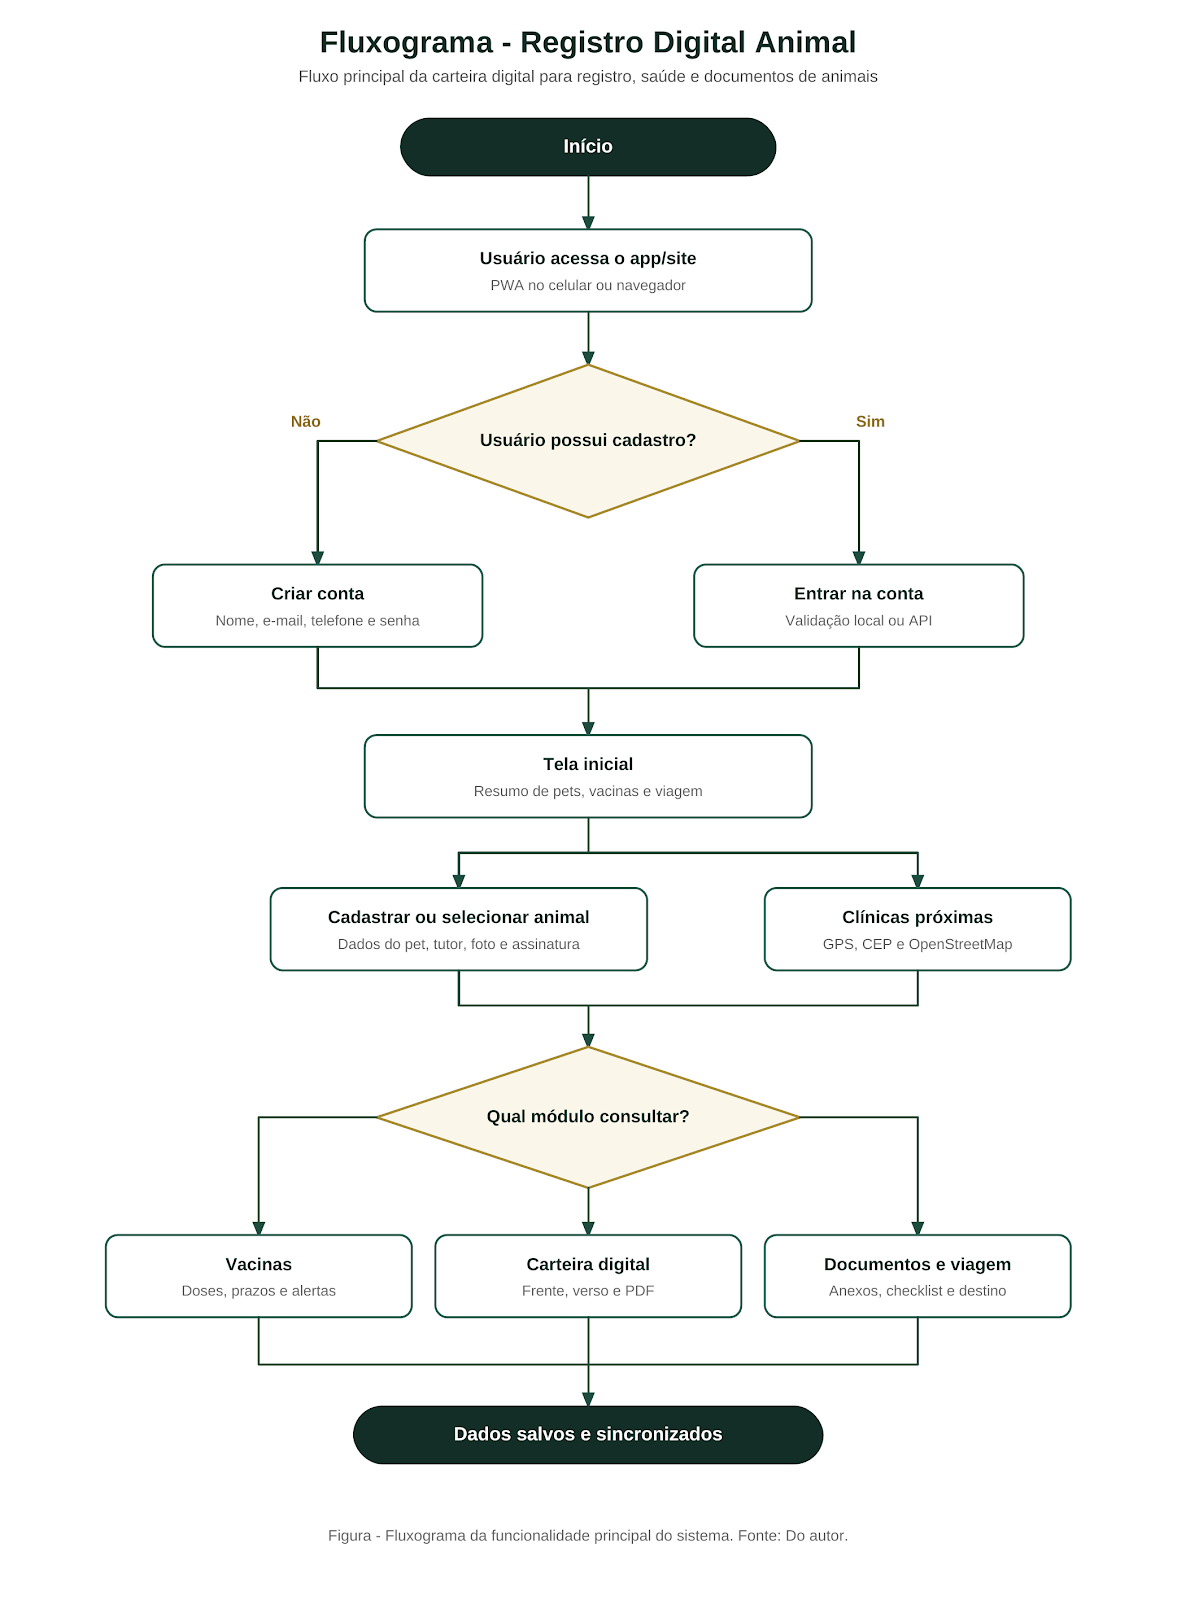
\includegraphics[scale=0.2]{Figs/fluxograma-registro-digital-animal.png}

\vspace{-0.2cm}
\begin{minipage}{\textwidth}
\footnotesize\raggedright Fonte: Elaborado pelo autor com auxílio do Codex GPT-5.5 (2026).
\end{minipage}
\end{figure}

No fluxo apresentado, o tutor acessa a aplicação por um navegador ou pela PWA instalada no dispositivo. As ações realizadas na interface são encaminhadas à API REST, responsável por processar as requisições, aplicar as regras do sistema e realizar as operações necessárias no banco de dados. As integrações externas são acionadas conforme a funcionalidade utilizada, enquanto os mecanismos de armazenamento local e sincronização permitem manter informações essenciais disponíveis em situações de conectividade limitada ou ausente.

Além do fluxo funcional, a Figura~\ref{fig:arquitetura_tecnologias_sistema} apresenta uma visão consolidada das tecnologias empregadas no desenvolvimento, na implantação e nos testes do sistema. O diagrama organiza os recursos utilizados nas camadas de \textit{frontend}, PWA e funcionamento offline, \textit{backend}, banco de dados, infraestrutura de hospedagem, integrações externas e ambiente de testes.

\begin{figure}[htbp]
\captionsetup{justification=raggedright,singlelinecheck=false,format=hang}
\caption{Arquitetura e tecnologias utilizadas no sistema Registro Digital Animal}
\label{fig:arquitetura_tecnologias_sistema}
\centering
\vspace{-0.2cm}
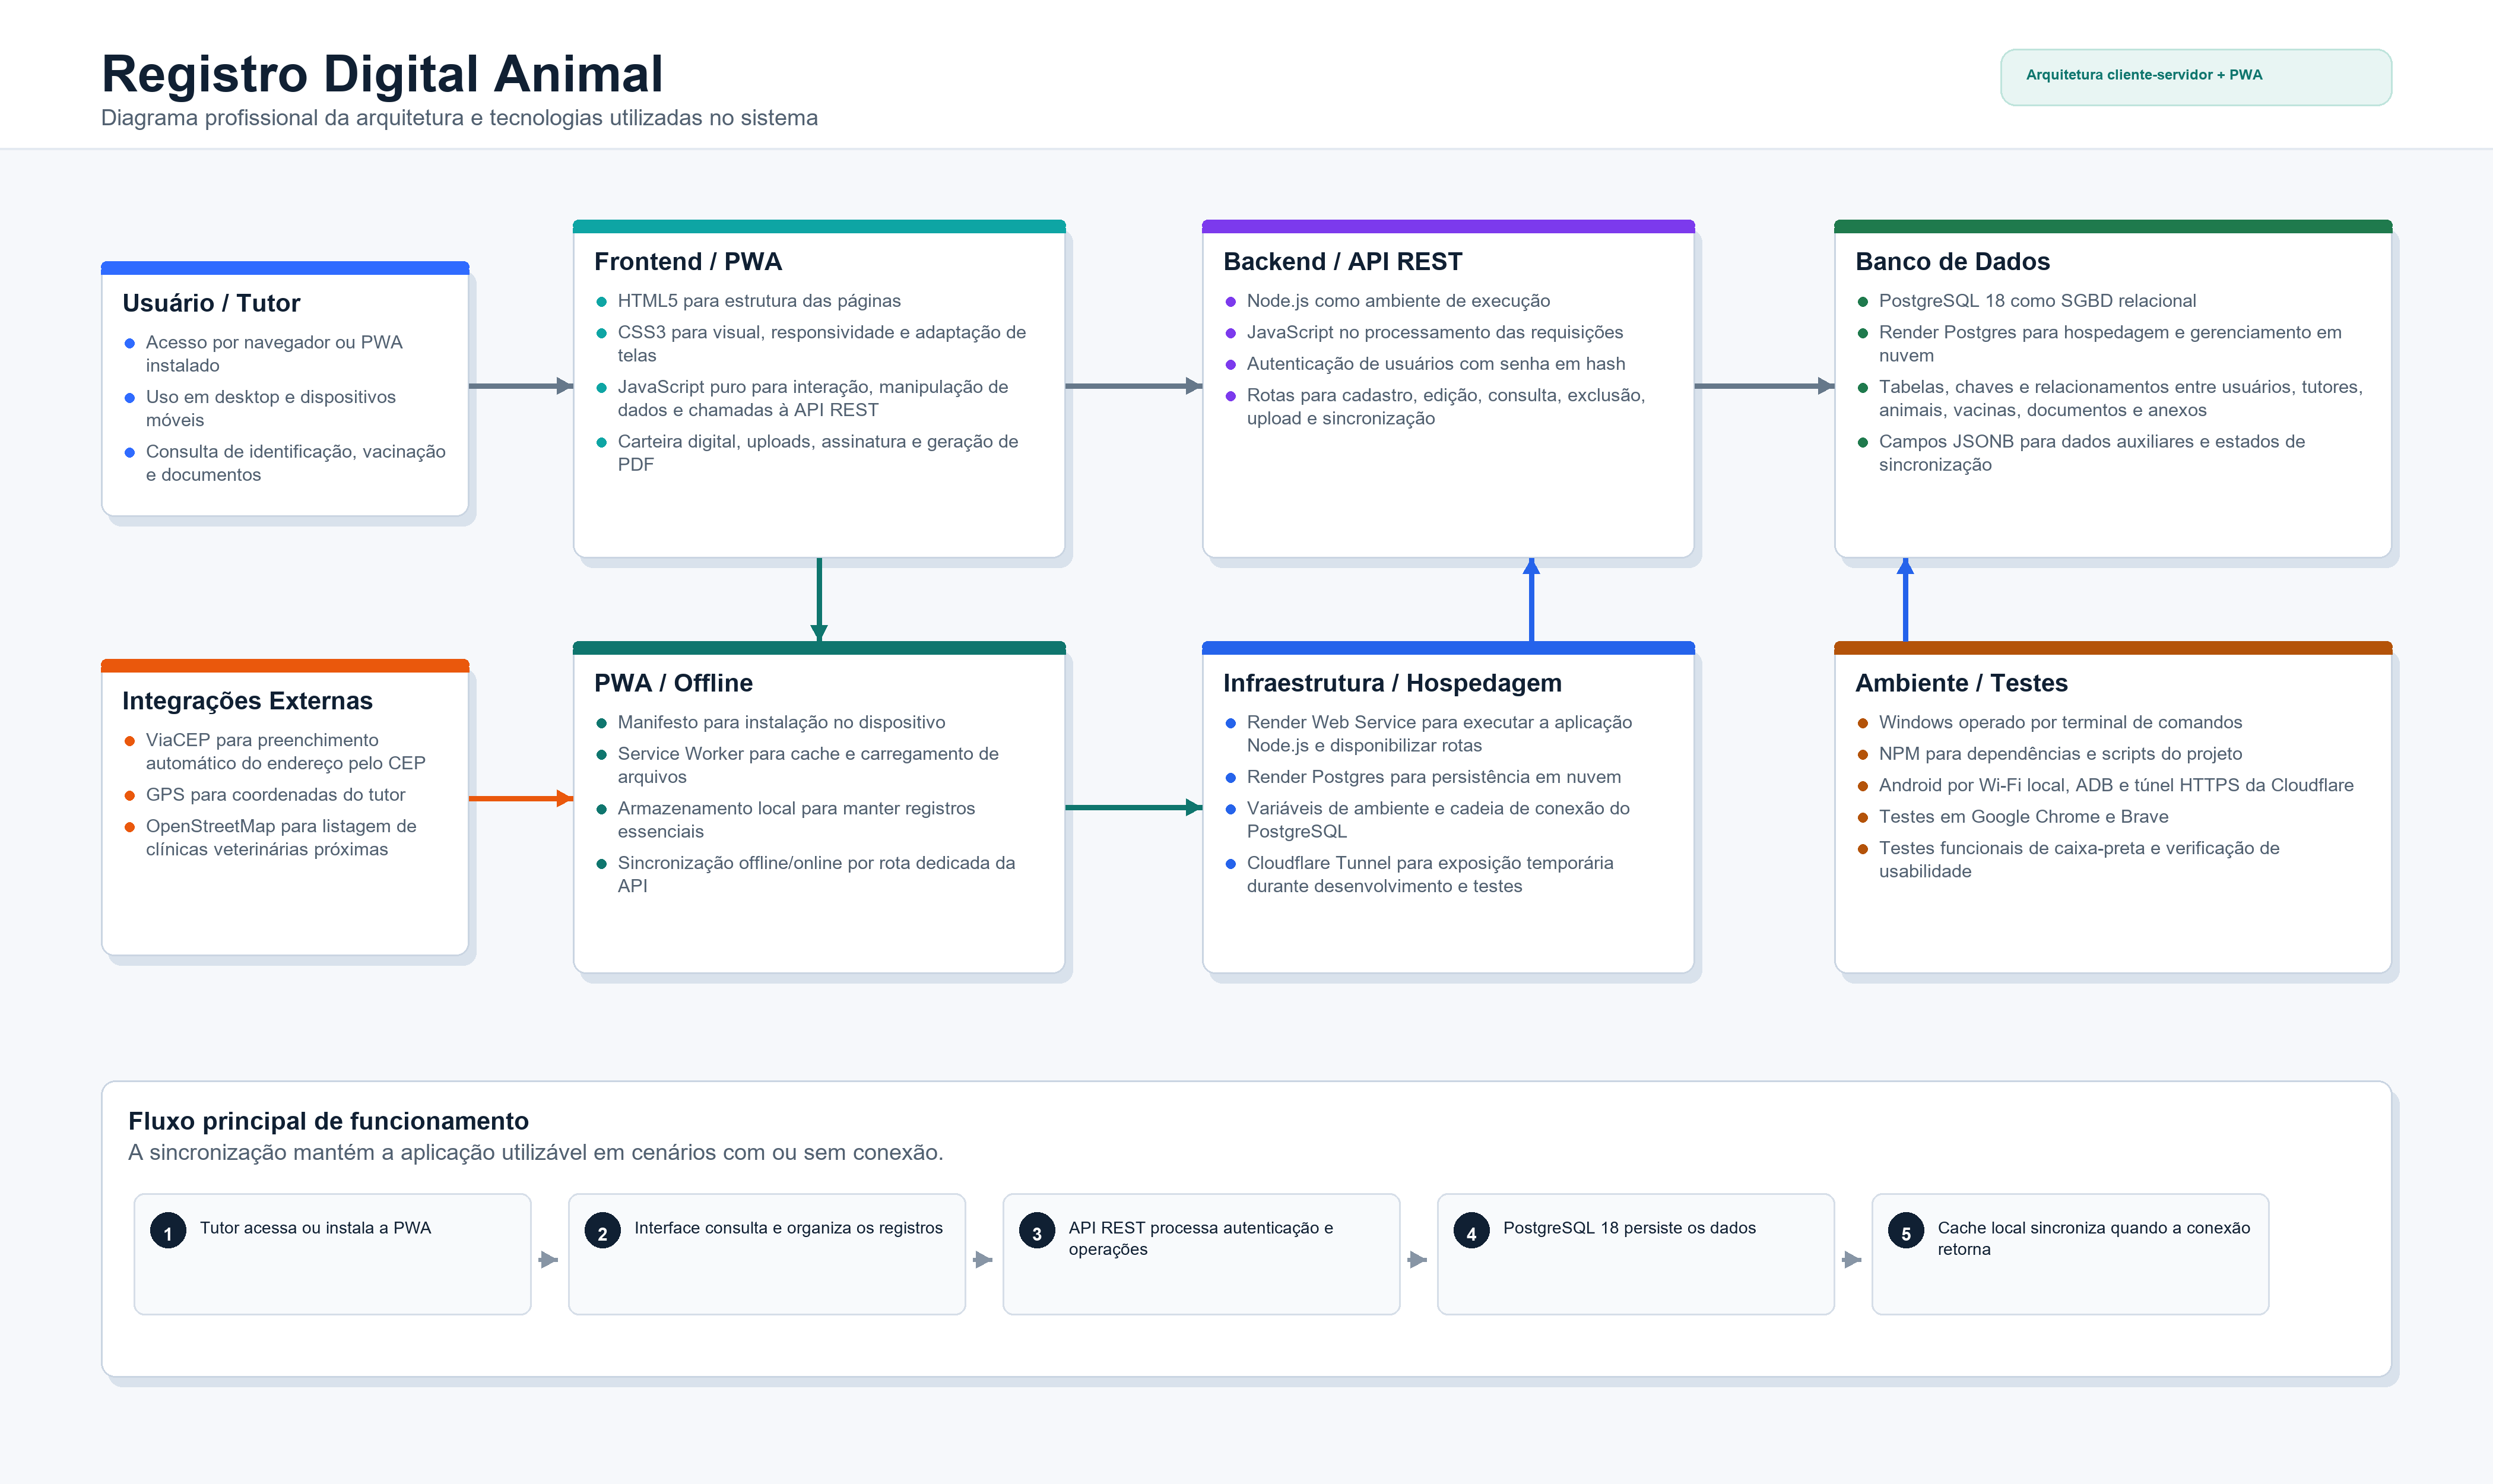
\includegraphics[width=\textwidth]{Figs/Registro_Digital_Animal_Diagrama.png}

\vspace{-0.2cm}
\begin{minipage}{\textwidth}
\footnotesize\raggedright Fonte: Elaborado pelo autor.
\end{minipage}
\end{figure}

No \textit{frontend}, foram utilizados HTML5, CSS3 e JavaScript puro, enquanto os recursos de PWA foram implementados por meio de manifesto, \textit{service worker}, \textit{cache} e armazenamento local. O \textit{backend} foi desenvolvido em JavaScript sobre o ambiente Node.js e organizado como uma API REST, com o NPM utilizado no gerenciamento das dependências e na execução dos scripts do projeto. A persistência das informações foi implementada no PostgreSQL 18. A infraestrutura descrita para a etapa de avaliação utilizou Render Postgres e Render Web Service. O projeto também contém configuração para publicação na Vercel e execução local. A comunicação com o banco foi parametrizada por variáveis de ambiente. A indisponibilidade posterior do banco hospedado limitou a recuperação de parte dos retornos da pesquisa de campo, conforme descrito na avaliação.

As integrações externas incluíram a API ViaCEP, utilizada no preenchimento automático de endereços, e os recursos de GPS e OpenStreetMap, empregados na localização de clínicas veterinárias próximas ao tutor. Durante o desenvolvimento e os testes, foram utilizados o sistema operacional Windows, os navegadores Google Chrome e Brave, dispositivos Android, rede local Wi-Fi, Android Debug Bridge (ADB) e túnel HTTPS da Cloudflare.

A aplicação foi composta por módulos voltados ao gerenciamento das informações do tutor e do animal. O módulo de usuários permitiu o cadastro e a autenticação na plataforma via API com senhas armazenadas em formato de \textit{hash}. O módulo de animais possibilitou registrar e editar os dados de identificação do pet, incluindo o \textit{upload} de foto e o preenchimento automático do endereço a partir da consulta do CEP por meio da API ViaCEP, permanecendo sob responsabilidade do usuário o preenchimento do número e do complemento.

Além disso, o sistema contou com uma carteira digital do animal visualizável em formato frente e verso, recursos para captura de assinatura digital diretamente na aplicação, \textit{upload} de documentos do pet em formato de imagem ou PDF e geração ou \textit{download} da carteira e de seus anexos compilados em formato PDF. Para auxiliar em situações de emergência e localização, a aplicação integrou a geolocalização por GPS do tutor e os dados do OpenStreetMap para listar clínicas veterinárias próximas.

\subsubsection{Banco de Dados}

A Figura~\ref{fig:diagrama_banco_dados} apresenta um recorte de seis tabelas do núcleo cadastral da aplicação. A implementação contém também estruturas auxiliares para itens de viagem, avaliações, estado sincronizado, anexos, sincronizações em partes e eventos de uso. Portanto, o diagrama não representa a totalidade do esquema. A descrição das seis estruturas representadas é apresentada a seguir.

\begin{itemize}
    \item \textbf{\texttt{pet\_app\_users}}: armazena as informações de cadastro e autenticação dos usuários, incluindo identificador, nome, e-mail, e-mail normalizado, telefone, \textit{hash} da senha e datas de criação e atualização. Seu identificador associa os registros ao usuário responsável.
    \item \textbf{\texttt{pet\_owners}}: mantém os dados do tutor vinculados ao usuário por \texttt{user\_id}, incluindo nome, CPF, telefone, e-mail, endereço, número, complemento, bairro, município, estado, CEP, coordenadas de localização e contato de emergência.
    \item \textbf{\texttt{pet\_pets}}: reúne os dados de identificação dos animais, associados ao usuário e identificados por \texttt{id}. Contempla nome, espécie, raça, sexo, nascimento, peso, cor, microchip, registro, temperamento, alergias, observações e cor de apresentação do perfil, além das datas de criação e atualização.
    \item \textbf{\texttt{pet\_vaccines}}: registra as vacinas relacionadas ao usuário e ao animal, por meio de \texttt{user\_id} e \texttt{pet\_id}. Contém identificador do registro, nome da vacina, dose, data de aplicação, data prevista para a próxima dose, clínica, veterinário, lote, observações e datas de criação e atualização.
    \item \textbf{\texttt{pet\_documents}}: organiza os documentos vinculados ao usuário e ao animal, armazenando título, categoria, data do documento, validade e observações. Também mantém os dados do anexo, como nome, tipo, tamanho, identificador de armazenamento, endereço do arquivo, indicadores e conteúdo do anexo, além das datas de envio, armazenamento, criação e atualização.
    \item \textbf{\texttt{pet\_travel\_plans}}: armazena o planejamento de viagem associado ao usuário e ao animal. Contempla destino, data da viagem, meio de transporte, identificação do animal selecionado, observações e data de atualização.
\end{itemize}

A Figura~\ref{fig:diagrama_banco_dados} apresenta as tabelas do recorte descrito, com os campos, tipos de dados, chaves e relacionamentos representados.

\begin{figure}[htbp]
\captionsetup{
    justification=raggedright,
    singlelinecheck=false,
    format=hang
}
\caption{Recorte do núcleo cadastral do banco PostgreSQL da aplicação Registro Digital Animal}
\label{fig:diagrama_banco_dados}

\centering
\vspace{-0.2cm}

\adjustbox{
    Clip=0pt 0pt {.38\width} 0pt,
    width=.62\textwidth
}{
    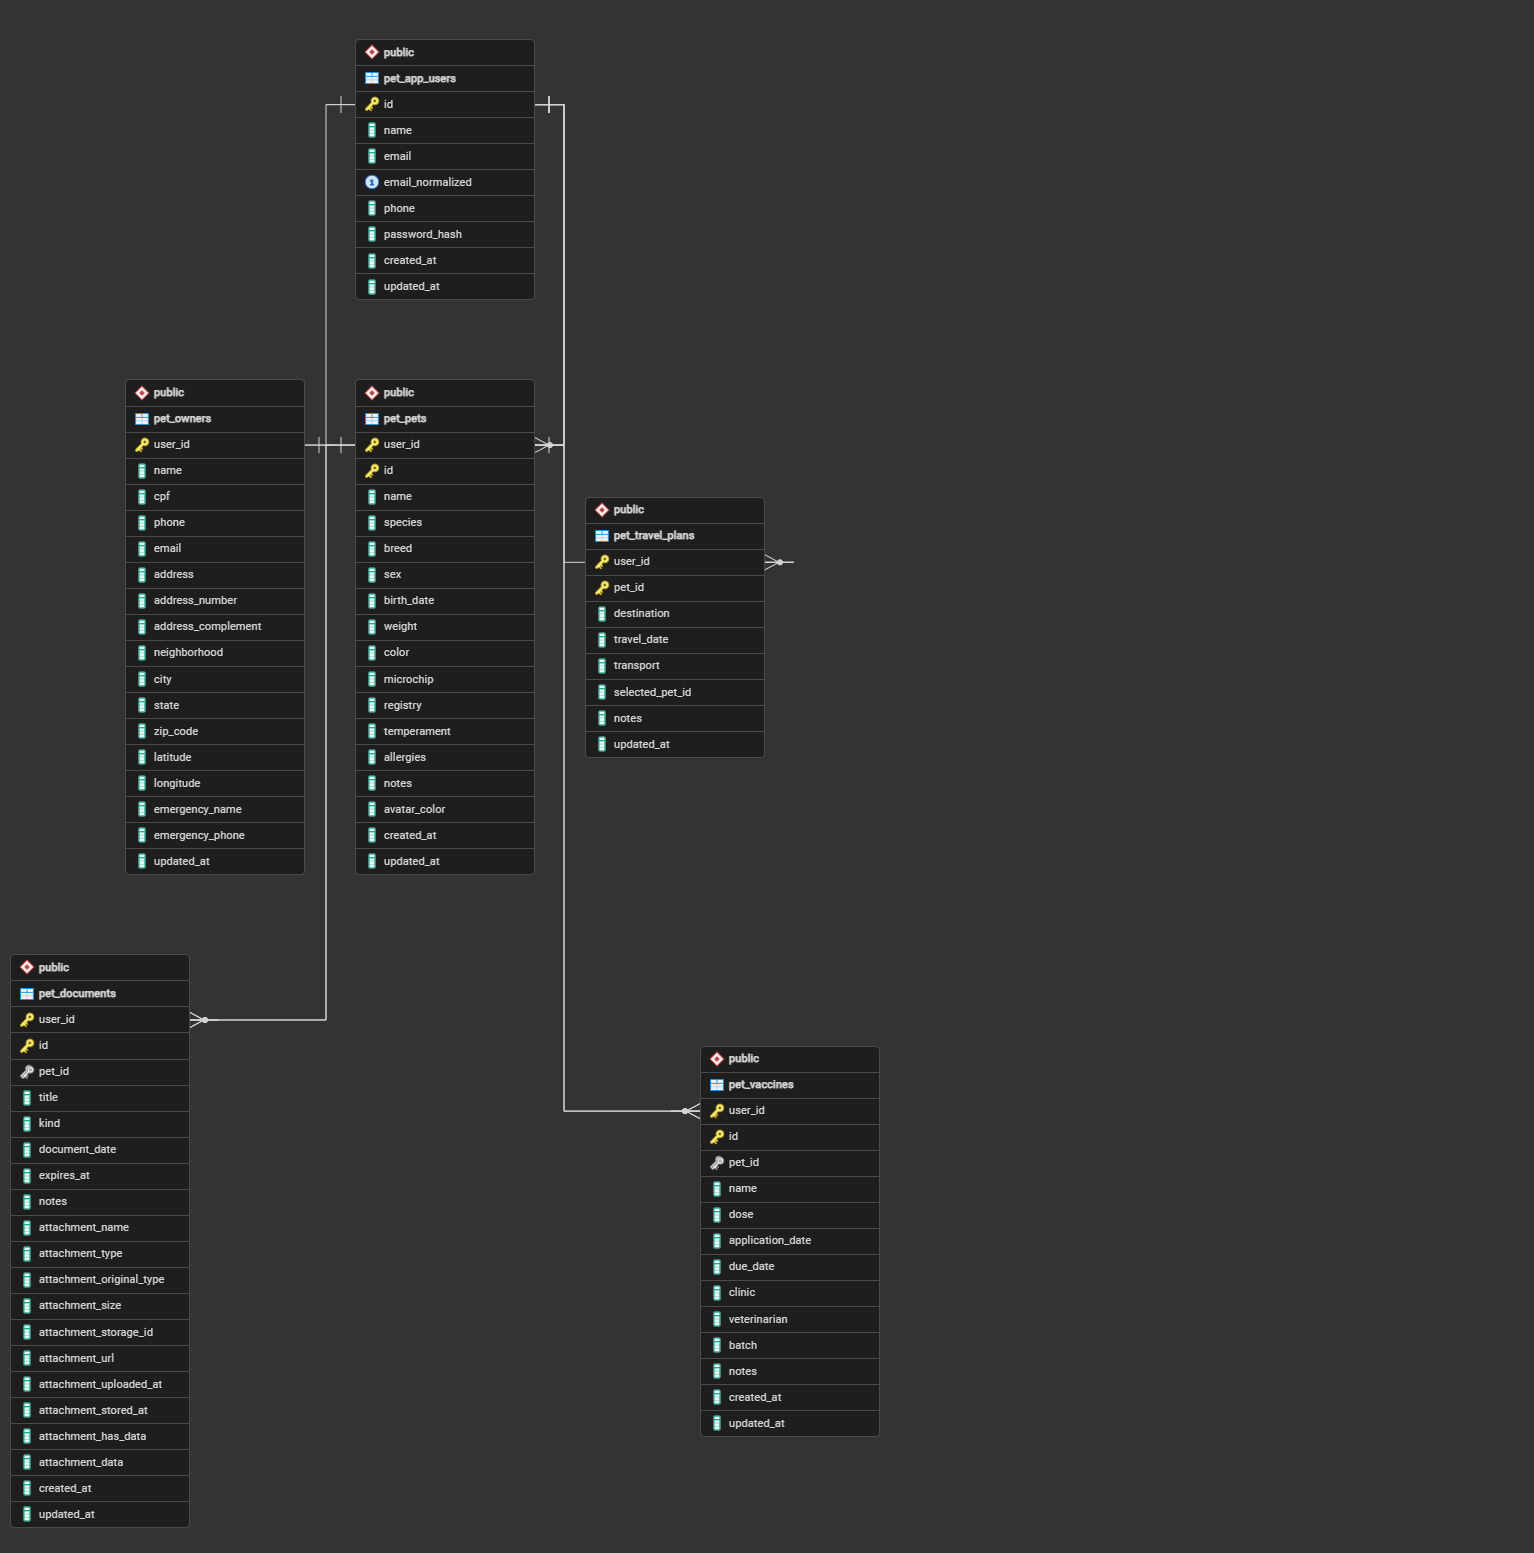
\includegraphics{Figs/Untitled.png}
}

\vspace{-0.2cm}
\begin{minipage}{\textwidth}
\footnotesize\raggedright
Fonte: Elaborado pelo autor.
\end{minipage}
\end{figure}

\subsection{Metodologia de Avaliação}

A avaliação compreendeu a verificação funcional de caixa-preta apresentada no desenvolvimento e a análise exploratória de retornos do setor veterinário. A verificação funcional comparou ações e resultados esperados. As observações sobre clareza das telas e navegação foram consideradas descritivas e não constituíram uma avaliação padronizada de usabilidade com usuários. A análise de retornos examinou utilidades percebidas e dificuldades relatadas, sem estimar aceitação populacional.

\subsubsection{Procedimento e cenários dos testes}

Os testes foram executados em computadores com Windows, nos navegadores Google Chrome e Brave, e em dispositivos Android. O acesso móvel foi realizado por rede local Wi-Fi, depuração USB com Android Debug Bridge (ADB) e túnel HTTPS da Cloudflare. Para cada cenário, comparou-se o comportamento observado ao resultado esperado. A classificação Passou correspondeu à execução da tarefa prevista e à manutenção dos dados envolvidos. A observação de usabilidade considerou clareza das telas, navegação, organização das informações e preenchimento dos formulários.

O conjunto de avaliação técnica descrito no estudo foi organizado em 15 cenários, identificados de F01 a F15 e relacionados aos resultados da Tabela~\ref{tab:testes_funcionais}. A classificação funcional se refere à tarefa prevista em cada cenário. Os registros não constituem uma bateria exaustiva de casos negativos, concorrência ou indisponibilidade de serviços, nem documentam medições de tempo, número de tentativas ou avaliações independentes de usabilidade. Os cenários foram:

\begin{itemize}
    \item \textbf{F01 -- Cadastro de usuário e armazenamento de senha com \textit{hash}}: Realizar o cadastro e verificar os dados persistidos e o armazenamento da senha em formato de hash.
    \item \textbf{F02 -- Autenticação do usuário e controle de sessão na API REST}: Efetuar o acesso e verificar a sessão e a restrição de acesso às rotas protegidas.
    \item \textbf{F03 -- Cadastro e edição de perfil de animal com \textit{upload} de foto}: Cadastrar e editar o animal, enviar uma fotografia e conferir os dados recuperados na interface.
    \item \textbf{F04 -- Preenchimento automático de endereço via API ViaCEP a partir do CEP}: Informar um CEP válido e conferir o preenchimento automático do endereço pela API ViaCEP.
    \item \textbf{F05 -- Captura e salvamento de assinatura digital no formulário}: Capturar e salvar a assinatura e verificar sua legibilidade e associação ao cadastro.
    \item \textbf{F06 -- Visualização interativa da carteira digital, com frente e verso}: Consultar a carteira e alternar entre frente e verso, conferindo os dados do tutor e do animal.
    \item \textbf{F07 -- \textit{Upload} e vinculação de documentos clínicos em imagem ou PDF}: Enviar documentos em imagem ou PDF e verificar a vinculação ao animal e a disponibilidade para consulta.
    \item \textbf{F08 -- Geração e exportação da carteira digital consolidada em PDF}: Gerar o PDF e conferir os dados cadastrais, vacinas, anexos e assinatura.
    \item \textbf{F09 -- Captura de coordenadas de geolocalização via GPS móvel}: Utilizar o GPS em Android e verificar a obtenção das coordenadas.
    \item \textbf{F10 -- Consulta de clínicas veterinárias próximas via OpenStreetMap}: Consultar os estabelecimentos no OpenStreetMap a partir da localização obtida.
    \item \textbf{F11 -- Responsividade e navegação em \textit{desktop} nos navegadores Chrome e Brave}: Navegar pelos principais fluxos em Chrome e Brave e verificar a adaptação às dimensões de tela.
    \item \textbf{F12 -- Acesso móvel em Android via Wi-Fi, ADB e túnel Cloudflare}: Comparar o acesso em Android por Wi-Fi, ADB e túnel HTTPS da Cloudflare.
    \item \textbf{F13 -- Armazenamento e execução de \textit{cache} pelo \textit{Service Worker}}: Verificar o armazenamento e o carregamento dos recursos da PWA pelo Service Worker.
    \item \textbf{F14 -- Acesso e consulta offline aos dados da carteira e das vacinas}: Interromper a conectividade e consultar os dados da carteira e das vacinas previamente armazenados.
    \item \textbf{F15 -- Sincronização offline-online de registros no banco PostgreSQL}: Realizar alterações locais sem conexão, restabelecer a conectividade e conferir o envio à API e a persistência no PostgreSQL.
\end{itemize}

A escala de severidade de Nielsen se destina à classificação de problemas de usabilidade identificados, considerando frequência, impacto e persistência \cite{nielsen1994}. Como não foi preservado um protocolo de julgamento independente desses fatores para cada cenário, não foram atribuídas notas de severidade nesta apresentação. A aprovação funcional foi mantida separada dos problemas e sugestões relatados pelos participantes.

\subsubsection{Procedimento da pesquisa de campo}

O convite à avaliação foi dirigido a clínicas, estabelecimentos e profissionais do setor animal, identificados pelo Google Maps em Criciúma e pela plataforma Casa dos Dados nas buscas para outros municípios. A seleção foi não probabilística e relacionada ao domínio da aplicação. A planilha de acompanhamento registrou 96 contatos, com datas de convite entre 11 e 18 de setembro de 2026. Predominaram localidades de Santa Catarina, mas um contato foi cadastrado com município Fortaleza; por isso, o conjunto de convites não foi tratado como exclusivamente catarinense. O contato ocorreu remotamente pelo WhatsApp, com apresentação do pesquisador e convite para conhecer e testar a aplicação. Aos que aceitaram, foram encaminhados o endereço do aplicativo e um vídeo de orientação. As mensagens solicitaram opinião sobre a experiência de uso, informações ausentes e possíveis melhorias.

Para caracterizar o recrutamento, foram considerados o status do convite, a data de envio do material e a marcação de feedback recebido na planilha. Os 96 contatos foram distribuídos em 13 aceites, 80 sem resposta e três sem interesse. Aceitar o convite, receber o material, cadastrar-se e enviar uma avaliação foram tratados como eventos distintos. A planilha indicou dois feedbacks recebidos, nas datas de 21 de setembro e 7 de outubro de 2026. Entre os demais aceites, dez permaneceram pendentes de feedback e um apresentou a observação de cadastro realizado sem avaliação. Esses registros não comprovam experimentação completa do aplicativo por todos os que aceitaram participar.

Além dos dois retornos assinalados na planilha, o pesquisador informou o recebimento de um terceiro, armazenado no banco hospedado no Render e indisponível para recuperação após a interrupção do serviço. Esse terceiro registro não apareceu como feedback recebido na planilha consultada e seu conteúdo não foi incluído na análise. Assim, o corpus analisado foi composto exclusivamente pelos dois retornos preservados. Os dois registros preservados foram identificados como R1 e R2, sem divulgação de nomes ou estabelecimentos. R1 correspondeu a uma avaliação estruturada salva pela aplicação, com notas e comentários; R2 correspondeu a um relato textual livre de uma participante que se referiu à rotina da medicina veterinária e informou ter cadastrado seus animais. O papel profissional específico de R1 não foi detalhado no registro disponível.

No formulário, os campos gerais registraram satisfação com as informações da carteira e avaliação do aplicativo. Os itens de concordância foram organizados em necessidade de melhoria da carteira, vacinação e viagens, além de utilidade de possíveis aprimoramentos nesses mesmos módulos. A concordância com a necessidade de melhoria não foi interpretada como satisfação. O relato livre foi examinado como percepção individual, sem conversão em pontuação.

A análise dos dois registros agrupou os comentários por conteúdo: organização e identificação do animal; preenchimento e informação vacinal; planejamento de viagens; localização de clínicas; e integração com a atuação veterinária. As menções foram associadas a R1 ou R2, permitindo rastrear cada interpretação ao registro correspondente. Não foram produzidas estimativas estatísticas ou frequências de aceitação. Os resultados apresentados limitam-se ao conteúdo preservado, e a categorização não foi submetida à concordância entre avaliadores independentes.

\begingroup
\makeatletter
\@ifundefined{captionsetup}{%
  \long\def\@makecaption#1#2{%
    \vskip\abovecaptionskip
    {\normalsize\normalfont
      \sbox\@tempboxa{#1\space-\space}%
      \raggedright
      \hyphenpenalty=10000
      \hangindent=\wd\@tempboxa
      \hangafter=1
      \noindent#1\space-\space#2\par}%
    \vskip\belowcaptionskip}%
}{%

  \captionsetup[table]{format=hang,justification=raggedright,
    singlelinecheck=false,labelsep=space,font=normalsize,
    labelfont=normalfont,textfont=normalfont,skip=6pt}%
}
\makeatother

\section{RESULTADOS E DISCUSSÃO}

Esta seção apresenta os resultados funcionais registrados para a aplicação \textbf{Registro Digital Animal} e a análise exploratória dos dois retornos preservados da pesquisa de campo. Os resultados são discutidos conforme o alcance de cada fonte: conclusão de tarefas nos cenários definidos e percepções individuais sobre utilidade e dificuldades de uso.

\subsection{Resultados dos cenários funcionais}

A Tabela~\ref{tab:testes_funcionais} apresenta os resultados dos 15 cenários definidos na seção de Materiais e Métodos. A classificação expressa o resultado funcional registrado, sem equivalência com uma medida de usabilidade.

\begin{table}[htbp]
\centering
\caption{Resultados registrados para os cenários funcionais do sistema}
\label{tab:testes_funcionais}
\par\vspace{4pt}
\small
\setlength{\tabcolsep}{4pt}
\renewcommand{\arraystretch}{1.15}
\begin{tabular}{@{}p{0.08\linewidth} p{\dimexpr0.76\linewidth-4\tabcolsep\relax} p{0.16\linewidth}@{}}
\hline
\textbf{ID} & \textbf{Cenário de teste avaliado} & \textbf{Resultado} \\
\hline
F01 & Cadastro de usuário e armazenamento de senha com \textit{hash} & Passou \\
F02 & Autenticação do usuário e controle de sessão na API REST & Passou \\
F03 & Cadastro e edição de perfil de animal com \textit{upload} de foto & Passou \\
F04 & Preenchimento automático de endereço via API ViaCEP a partir do CEP & Passou \\
F05 & Captura e salvamento de assinatura digital no formulário & Passou \\
F06 & Visualização interativa da carteira digital, com frente e verso & Passou \\
F07 & \textit{Upload} e vinculação de documentos clínicos em imagem ou PDF & Passou \\
F08 & Geração e exportação da carteira digital consolidada em PDF & Passou \\
F09 & Captura de coordenadas de geolocalização via GPS móvel & Passou \\
F10 & Consulta de clínicas veterinárias próximas via OpenStreetMap & Passou \\
F11 & Responsividade e navegação em \textit{desktop} nos navegadores Chrome e Brave & Passou \\
F12 & Acesso móvel em Android via Wi-Fi, ADB e túnel Cloudflare & Passou \\
F13 & Armazenamento e execução de \textit{cache} pelo \textit{Service Worker} & Passou \\
F14 & Acesso e consulta offline aos dados da carteira e das vacinas & Passou \\
F15 & Sincronização offline-online de registros no banco PostgreSQL & Passou \\
\hline
\end{tabular}
\par\vspace{2pt}
\begin{minipage}{\linewidth}
\footnotesize\raggedright
Fonte: Elaborado pelo autor.
\end{minipage}
\end{table}

Os 15 cenários funcionais definidos foram registrados como aprovados nas condições de teste descritas. Esse resultado se restringe às tarefas previstas e não caracteriza ausência de falhas em outros cenários, nem substitui uma avaliação de usabilidade com usuários. O conjunto não permite estimar confiabilidade em produção ou taxas de sucesso para uma população de tutores.

Nos cenários F01 e F02, referentes à autenticação e ao controle de acesso, verificou-se que a API REST realizou corretamente o cadastro de usuários, armazenando as senhas em formato de \textit{hash}, conforme a implementação de autenticação do servidor. Também foi confirmada a restrição de acesso às rotas protegidas, o que contribui para a segurança dos dados pessoais e dos registros dos animais.

No módulo de gestão do animal, contemplado pelos cenários F03 a F05, o formulário de cadastro apresentou comportamento consistente durante a inserção e edição das informações. A integração com a API ViaCEP reduziu o preenchimento manual de dados de endereço, ao completar automaticamente logradouro, bairro, cidade e estado após a inserção de um CEP válido. A captura da assinatura digital também foi executada corretamente, mantendo a legibilidade do traço e sua associação ao cadastro do animal.

Em relação à carteira digital e aos documentos, avaliados nos cenários F06 a F08, a aplicação permitiu a visualização organizada das informações do animal e do tutor, incluindo a alternância entre frente e verso da carteira. O envio de documentos clínicos em imagem ou PDF funcionou adequadamente, e a exportação consolidada em PDF reuniu os principais dados cadastrais, registros de vacinação, anexos e assinatura digital em um único arquivo. Esse resultado reforça a proposta do sistema como alternativa digital à caderneta física, especialmente em situações nas quais o tutor precisa apresentar rapidamente o histórico do animal.

Os testes de mobilidade e geolocalização, correspondentes aos cenários F09 a F12, demonstraram que a aplicação manteve comportamento estável em diferentes formas de acesso. Em dispositivos Android, a captura de coordenadas por GPS e a integração com o OpenStreetMap possibilitaram a listagem de estabelecimentos veterinários próximos à localização do usuário. Além disso, a execução em rede Wi-Fi local, depuração via ADB e acesso por túnel HTTPS com Cloudflare apresentou funcionamento equivalente, sem inconsistências relevantes de navegação ou renderização da interface.

Por fim, os cenários F13 a F15 validaram os recursos de funcionamento offline e sincronização posterior. O \textit{Service Worker} e os mecanismos de \textit{cache} permitiram que a aplicação permanecesse acessível mesmo na ausência de conexão com a internet, permitindo, nos cenários descritos, a consulta às informações essenciais da carteira e dos registros de vacinação já salvos no dispositivo. Quando a conectividade foi restabelecida, os registros pendentes foram enviados à API REST e persistidos no banco PostgreSQL, evidenciando a viabilidade do uso da aplicação em contextos de mobilidade, atendimento externo ou instabilidade de rede.

Embora os resultados tenham sido positivos, ressalta-se que os testes foram realizados em um conjunto controlado de cenários e dispositivos. Assim, avaliações futuras com maior diversidade de usuários, navegadores, modelos de aparelhos e condições de conectividade podem ampliar a confiabilidade da validação e revelar necessidades adicionais de aprimoramento.

\subsection{Análise dos retornos preservados da pesquisa de campo}

O registro de recrutamento apresentou 13 aceites entre 96 contatos, equivalentes a 13,5\% dos convites registrados. Os 80 contatos sem resposta e as três manifestações de desinteresse indicam que a obtenção de participação exigiu alcançar um conjunto maior de potenciais avaliadores. Entre os 13 aceites, somente dois tiveram feedback marcado como recebido. Esses números descrevem o acompanhamento dos convites e não constituem uma medida de satisfação ou de utilização efetiva. A Tabela~\ref{tab:recrutamento} resume as etapas documentadas.

\begin{table}[htbp]
\centering
\caption{Situação dos contatos e disponibilidade dos retornos para análise}
\label{tab:recrutamento}
\small
\setlength{\tabcolsep}{5pt}
\renewcommand{\arraystretch}{1.15}
\begin{tabular}{@{}p{\dimexpr0.84\linewidth-2\tabcolsep\relax} r@{}}
\hline
\textbf{Etapa ou situação registrada} & \textbf{Quantidade} \\
\hline
Contatos com convite registrado & 96 \\
Aceitaram participar & 13 \\
Sem resposta ao convite & 80 \\
Não interessados & 3 \\
Aceites com feedback marcado como recebido & 2 \\
Aceites com feedback pendente & 10 \\
Aceite com cadastro, sem feedback, conforme observação & 1 \\
Retornos preservados incluídos na análise & 2 \\
Retorno adicional informado, indisponível e excluído & 1 \\
\hline
\end{tabular}
\par\vspace{2pt}
{\footnotesize\raggedright Fonte: Elaborado pelo autor a partir da planilha de acompanhamento e dos registros preservados. As linhas representam etapas e subconjuntos; não devem ser somadas como categorias independentes.\par}
\end{table}

Os dois retornos preservados apresentaram conteúdos distintos e complementares. R1 reuniu notas e comentários específicos sobre campos da aplicação; R2 apresentou um relato livre sobre sua utilidade e possíveis ampliações. A Tabela~\ref{tab:resumo_qualitativo} relaciona os aspectos analisados aos registros que os sustentam. As descrições correspondem a menções individuais, sem indicação de prevalência entre profissionais veterinários.

\begin{table}[htbp]
\centering
\caption{Síntese dos comentários presentes nos dois retornos preservados}
\label{tab:resumo_qualitativo}
\small
\setlength{\tabcolsep}{4pt}
\renewcommand{\arraystretch}{1.15}
\begin{tabular}{@{}p{0.24\linewidth} p{\dimexpr0.66\linewidth-4\tabcolsep\relax} p{0.10\linewidth}@{}}
\hline
\textbf{Aspecto} & \textbf{Comentário ou sugestão registrada} & \textbf{Fonte} \\
\hline
Identificação e preenchimento & Dificuldade para informar o peso de 16,3; valorização de informações mais detalhadas sobre o animal. & R1 \\
Registro de vacinas & Questionamento sobre a necessidade do campo de quantidade de aplicação, considerado assunto de análise veterinária. & R1 \\
Organização e consulta & Utilidade dos dados para preenchimento pelo tutor e comunicação das informações durante o atendimento; navegação descrita como fácil. & R2 \\
Identificação por microchip & Valorização do registro de microchip como informação útil em situações de resgate. & R2 \\
Planejamento de viagens & Área descrita como completa e útil para organização antecipada de documentos. & R2 \\
Localização de clínicas & Utilidade da busca de estabelecimentos próximos e sugestão de destacar os que atendem 24 horas. & R2 \\
Atuação veterinária & Sugestão de área profissional com identificação pelo registro de conselho, consulta por microchip e registros de atendimento. & R2 \\
\hline
\end{tabular}
\par\vspace{2pt}
{\footnotesize\raggedright Fonte: Elaborado pelo autor a partir dos retornos preservados.\par}
\end{table}

Em R1, os campos gerais apresentaram nota 5 para as informações da carteira e nota 4 para a avaliação do aplicativo, em escala de 1 a 5. Essas duas notas pertencem a um único retorno e não foram tratadas como média de satisfação da amostra. Os itens adicionais de concordância avaliaram necessidade de melhoria e utilidade de aprimoramentos; por isso, suas notas não foram agregadas às avaliações gerais. A leitura dos comentários foi necessária para compreender as dificuldades concretas relatadas.

A dificuldade com peso decimal apareceu no exemplo de um animal com 16,3, cujo peso foi registrado como 16 porque o valor exato não foi aceito na interação descrita por R1. Esse achado evidencia uma limitação percebida no preenchimento, sem permitir atribuir sua causa ao navegador, à versão do aplicativo ou à validação de um campo específico. O comentário sobre quantidade de aplicação também indica a necessidade de revisar a clareza e a pertinência dos dados solicitados no módulo de vacinação, considerando a distinção entre registro pelo tutor e avaliação profissional.

R2 destacou a organização das informações e a facilidade para localizá-las na interface. A participante afirmou ter cadastrado seus animais e considerou úteis os dados de identificação, o registro de microchip, o planejamento de viagens e a busca de clínicas próximas. A observação sobre destacar estabelecimentos com atendimento 24 horas indica que a proximidade geográfica, isoladamente, pode ser insuficiente para orientar uma busca em situação de urgência. Trata-se de uma necessidade identificada no relato, sem comprovação de redução de tempo de atendimento ou melhoria de desfechos clínicos.

A sugestão de uma área veterinária, com consulta por microchip e registros de atendimento, amplia o problema para o compartilhamento de informações entre tutores e profissionais. Sua implementação exigiria investigar responsabilidades, autorização de acesso e verificação de identidade profissional. A menção a um número de conselho, por si só, não demonstra um mecanismo suficiente de validação de identidade. A sugestão foi mantida como possibilidade de investigação e não como funcionalidade já entregue.

R2 relacionou a organização digital ao acompanhamento das datas de revacinação. Esse comentário permite discutir a relevância percebida de acompanhar prazos, mas não demonstra que notificações automáticas tenham sido implementadas ou avaliadas. Da mesma forma, não foram identificados nos dois retornos comentários específicos que comprovem aceitação do funcionamento offline ou da exportação em PDF. Esses recursos foram descritos na avaliação técnica; sua apreciação pelos participantes não foi presumida.

\subsection{Limitações e ameaças à validade}

A avaliação funcional se limitou aos cenários e ambientes descritos, sem cobertura exaustiva de entradas inválidas, falhas de serviços externos, conflitos entre dispositivos ou perda de conexão durante o envio de anexos. A ausência de medidas de tempo, repetição e comparação com outra solução restringe conclusões sobre desempenho e facilidade de uso. A observação realizada no contexto de desenvolvimento também pode favorecer familiaridade com os fluxos, reduzindo a identificação de dificuldades enfrentadas por novos usuários.

Na pesquisa de campo, a seleção por conveniência, a análise de apenas dois retornos preservados, a caracterização incompleta dos respondentes e a combinação de formulário estruturado com relato livre limitam a comparação entre participantes. A indisponibilidade do terceiro retorno introduziu perda de dados, cujo efeito sobre o conjunto de opiniões não pôde ser avaliado. A diferença entre aceites e retornos preservados introduz viés de não resposta: as percepções disponíveis podem não representar os profissionais que não responderam ou que aceitaram sem enviar avaliação. O retorno adicional informado pelo pesquisador não foi incorporado às contagens documentadas na planilha, evitando presumir a atualização desse registro. A categorização por um único analista também admite viés de interpretação.

Os resultados não demonstram redução efetiva do uso de registros físicos, aumento de adesão à vacinação ou superioridade em relação a aplicativos existentes. A assinatura capturada no aplicativo e o documento exportado constituem recursos de registro e apresentação; a pesquisa não avaliou autenticação da autoria ou aceitação documental por terceiros. Essas limitações delimitam a contribuição como desenvolvimento de um artefato e avaliação exploratória de seu funcionamento e de necessidades percebidas.

\endgroup

\section{CONCLUSÃO}

Este trabalho abordou a organização de informações de identificação, vacinação e documentos clínicos de animais de estimação por meio da aplicação multiplataforma Registro Digital Animal. O objetivo de desenvolver e avaliar o funcionamento da solução foi atendido no âmbito dos módulos implementados e dos cenários funcionais descritos. A aplicação reuniu cadastro de tutores e animais, carteira digital, registros vacinais, documentos e recursos de consulta em computadores e dispositivos móveis, incluindo acesso a informações previamente armazenadas e sincronização posterior.

Os 15 cenários funcionais foram registrados como aprovados nas condições avaliadas. Esse resultado indica atendimento às tarefas previstas, mas não comprova ausência de falhas nem usabilidade generalizável. Os dois retornos preservados complementaram a avaliação técnica ao apontarem utilidade na organização dos dados e no planejamento de viagens, juntamente com dificuldades e necessidades específicas: preenchimento de peso decimal, pertinência dos campos vacinais, identificação de clínicas com atendimento 24 horas e possibilidades de participação profissional.

A contribuição prática foi a construção de um artefato que reuniu diferentes registros do animal em uma interface acessível ao tutor. Como contribuição ao conhecimento no contexto estudado, a avaliação exploratória mostrou a necessidade de considerar conjuntamente a disponibilidade da informação, a precisão do preenchimento e sua adequação ao uso profissional. A aprovação de fluxos funcionais não eliminou dificuldades relatadas por participantes, o que reforça a importância de complementar testes técnicos com observação do uso. O estudo oferece, assim, requisitos e questões para novas avaliações, sem afirmar uma generalização teórica ou superioridade da solução.

O alcance dessas contribuições foi limitado pelo conjunto de testes, pela ausência de comparação com registros físicos e pela análise de somente dois retornos preservados, embora houvesse 13 aceites entre os 96 convites registrados e informação de um retorno adicional indisponível. A perda de acesso ao terceiro retorno restringiu a rastreabilidade da coleta. Além disso, a seleção não probabilística e a caracterização parcial dos participantes impedem estender suas percepções a todos os tutores ou profissionais. A redução da dependência de documentos físicos permaneceu como benefício pretendido, sem mensuração de sua ocorrência.

Uma lição do estudo foi que o armazenamento remoto não dispensa procedimentos de preservação dos dados de avaliação. A indisponibilidade de um registro evidenciou a necessidade de cópias independentes e de documentação do processo de coleta. Outra lição foi distinguir correção de uma operação, clareza da interface e utilidade percebida: essas dimensões podem apresentar resultados diferentes e exigem evidências próprias. Tais cuidados são aplicáveis a outros projetos que associem desenvolvimento de software e avaliação exploratória com participantes.

Como trabalhos futuros, propõe-se investigar, com tutores e veterinários de perfis distintos, se a carteira digital altera o tempo de localização das informações, a completude dos registros e a frequência de consulta quando comparada à documentação física. Estudos de uso ao longo do tempo poderão examinar a manutenção do histórico e o acompanhamento de prazos vacinais. Também se recomenda avaliar cenários de conectividade intermitente, edições concorrentes e recuperação de dados para compreender em quais condições a sincronização mantém informações consistentes. A participação veterinária e a busca de clínicas em situações de urgência constituem outras questões de pesquisa, envolvendo qualidade dos dados, autorização de acesso e confiabilidade da informação apresentada.

Conclui-se que a aplicação constituiu uma alternativa tecnicamente implementada para centralizar os registros no contexto delimitado, acompanhada de evidências iniciais de funcionamento e de necessidades de aprimoramento. A continuidade da pesquisa deverá verificar seus efeitos no uso cotidiano e ampliar a base empírica necessária para avaliar sua contribuição à organização das informações dos animais.

\bibliographystyle{abntex2-unesc}
\renewcommand{\refname}{REFERÊNCIAS}
\bibliography{referencias} % arquivo referencias.bib que contém as referências bibliográficas utilizadas no artigo

\end{document}
